\subsubsection{Spearman plots}
One interesting thing to note about nearly all of the Spearman plots is that there seem to be several clusters of proteins. Unfortunately, the dataset with stability scores does not also have a structural classification or similar to compare with. It would be quite interesting to see whether some of the structural classes are more difficult to predict the stability of. This is especially clear in Figure ~\ref{fig:cluster_spearman}. Another interesting note is that the better performing models seem to not have as many small clusters. This can be seen in Figure ~\ref{fig:small_cluster_spearman}.

\subsubsection{Training loss}
While working on this project, we noticed a weird phenomenon with both the LSTM and the CNN models while training. There seem to be large local minima at some specific points that nearly all the models hit during training. For the LSTM, this minimum seems to be when the model hits a training loss of around $2.8$. If we stop a model that only got to this point, it will usually predict almost entirely the most common amino acid. One of the experiments only barely got past this point, as can be seen in Figure: ~\ref{fig:predictions}. For comparison, the loss logs of this model, with 1-layer and $256$ features and the $1024$ model can be seen in Figure ~\ref{fig:loss_weird}.

\begin{figure}[!ht]
  \centering
  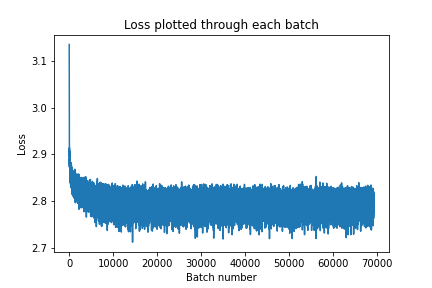
\includegraphics[width=0.49\linewidth]{latex/imgs/loss_log_1_layer_with_schedule_256.png}
  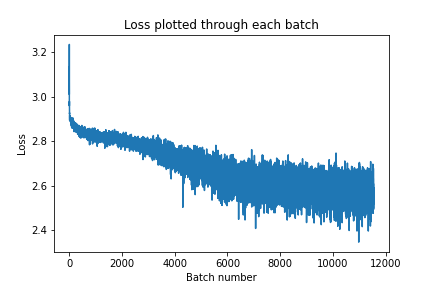
\includegraphics[width=0.49\linewidth]{latex/imgs/loss_log_1_layer_with_schedule_1024.png}
  \caption{Example showing the very different loss logs. The left plot shows the $256$ model, and the right shows the $1024$ model. Note the y-axis values.}
  \label{fig:loss_weird}
\end{figure}